\documentclass[../thesis.tex]{subfiles}
% Separate preamble for this subfile. This preamble is loaded last, so one can override various functions before \begin{document}

% Better comment extension for Vscode colors these comments differently
% Normal comment color
% * Important information
% ! ALERT
% ? Question
% TODO stuff to do
% // This is strikethrough


\begin{document}
%* ———————————————————————————— One dimension  ——————————————————
%* Viktig, må inn en bit her om 
%* som en konsekvens av Kellers theorem så får vi nå akkurat den samme formen på disse tilings settene 
%* de må ligge inneholt i akkurat de samme typene mengder, og de kan ikke være ekte mindre for da får vi ikke oppfylt tiling kravet mitt.
If we now restrict our attention to tilings of the unit cube in $\R^d$, Keller's \namecref{thrm:keller_tiling} immediately gives the following for dimension one.  For $d=1$, the unit cube is simply the unit interval $I = \bras{0,1}$. %In dimension one, the unit cube is simply the unit interval $I = \bras{0,1}$. 

\begin{lemma}\label{lem:tiling_unit_1d}
    %The set $\Lambda = \Z +\alpha$ for some value $\alpha\in \R$ constitutes a tiling set for $I$.
    %The only subsets $\Lambda \in \R$ such that $\Lambda$ is a tiling set for $I$ are $\Lambda = \Z +\alpha$ for some value $\alpha\in \R$.
    The only subsets $\Lambda \in \R$ such that $\Lambda$ is a tiling set for $I$ are the translates $\Lambda = \Z +\alpha$ for a fixed value $\alpha\in \R$. 
\end{lemma}

\begin{proof}  % This follows directly from \cref{thrm:keller_tiling}. Take $\lambda, \lambda' \in \Lambda$. 
    %  Må konkret gå tilbake til definisjonen du har valgt. For den kan vi bruke eksplisitt til å si:
    %Det Keller's theorem forteller meg, er at jeg må ha noe som er en undermengde av $\Lambda = \Z + \alpha$, og i og med at jeg må ha 1 almost everywhere, så gjør det at hvis jeg tar bort et punkt fra $\Lambda$ slik at vi har $\Lambda \subset \Z + \alpha$, så vil jeg få et intervall hvor jeg har 0.
    %  La oss nå si at et punkt er utelatt. Det betyr at $\sum \indicator{\Omega}{t} = 0$ og vi kan si nøyaktig hvor det er null, for det er på det punktet vi har utelatt. Dvs, $x\in I+\lambda'$, hvor $\lambda'$ er punktet vi utelot fra flisleggingsmengden. Videre, så er målet av $I+\lambda'$ positivt, det er ikke neglisjerbart. Dvs, der du ikke har verdien 1, de områdene, de er ikke neglisjerbare. Og videre vet vi at vi har $x\in I+\lambda'$, dvs et helt slikt interval, hvor $\sum \indicator{\Omega}{t} = 0$, og dette området har positivt mål. 
    Let $\Lambda \subset \R^d$. Using Keller's \namecref{thrm:keller_tiling}, \cref{thrm:keller_tiling}, we instantly get that there must be an integer distance between two distinct points $\lambda,\lambda' \in \Lambda$ if $\Lambda$ is to be a tiling set for $I$. Hence, we know that $\Lambda \subseteq \Z +\alpha$ for a fixed $\alpha\in \R$. Now, given an arbitrary point $\lambda' \in \Z +\alpha$, assume that $\lambda'\notin \Lambda$ so that we have a case where $\Lambda \subset \Z+\alpha$. However, by using \cref{def:tiling}, observe now that we have an entire interval, specifically $I+\lambda'$, where $\indicator{I}{x - \lambda'} = 0$. As $\mes{I+\lambda'} = 1 $, this is non-negligible, and we do not achieve
    \begin{equation*}
        \sum_{\lambda \in \Lambda\setminus \braq{\lambda'}} \indicator{I}{x-\lambda} = 1, \quad a.e. \text{\space\space} x \in \R^d.
    \end{equation*}
    %* As $\mes{I+\lambda'} = 1 $, this is non-negligible, and we do not achieve $\indicator{I}{x-\lambda} = 1$ almost everywhere for $x\in\R^d$ with the set $\Lambda\setminus \braq{\lambda'}$. % In short: That is, we have a non-negligible region with a value not equal to one.
    Hence $\lambda' \in \Lambda$, which shows that $\Lambda = \Z+\alpha$. This concludes the proof that there are no other tiling sets for $I$ in dimension $d=1$. %and that $\Lambda$ is a tiling set for $I$ . %for a tiling set $\Lambda$ of
\end{proof}

Increasing the dimension by one, we get more flexibility. In particular, when $d=2$, we do not necessarily need to have a lattice tiling as the one in \cref{fig:tiling_one}. We can have tilings where we translate single or multiple \emph{columns} of the unit cube, shown in \cref{fig:single_shift_vertical_tiling,fig:multiple_shift_vertical_tiling}; or single or multiple \emph{rows} of the unit cube, shown in \cref{fig:single_shift_horizontal_tiling,fig:multiple_shift_horizontal_tiling}. We will see later in \cref{chap:equivalence} that \cref{fig:tiling_figures} to some extent fully captures the flexibility of two dimensions. We remark that all \cref{fig:single_shift_vertical_tiling,fig:multiple_shift_vertical_tiling,fig:single_shift_horizontal_tiling,fig:multiple_shift_horizontal_tiling} clearly illustrates that all tilings of the unit cube in $\R^2$ also satisfy Keller's \namecref{thrm:keller_tiling}. 




\begin{figure}[t!]%h!
    \centering
    \begin{subfigure}{.47\textwidth}
        \centering
        %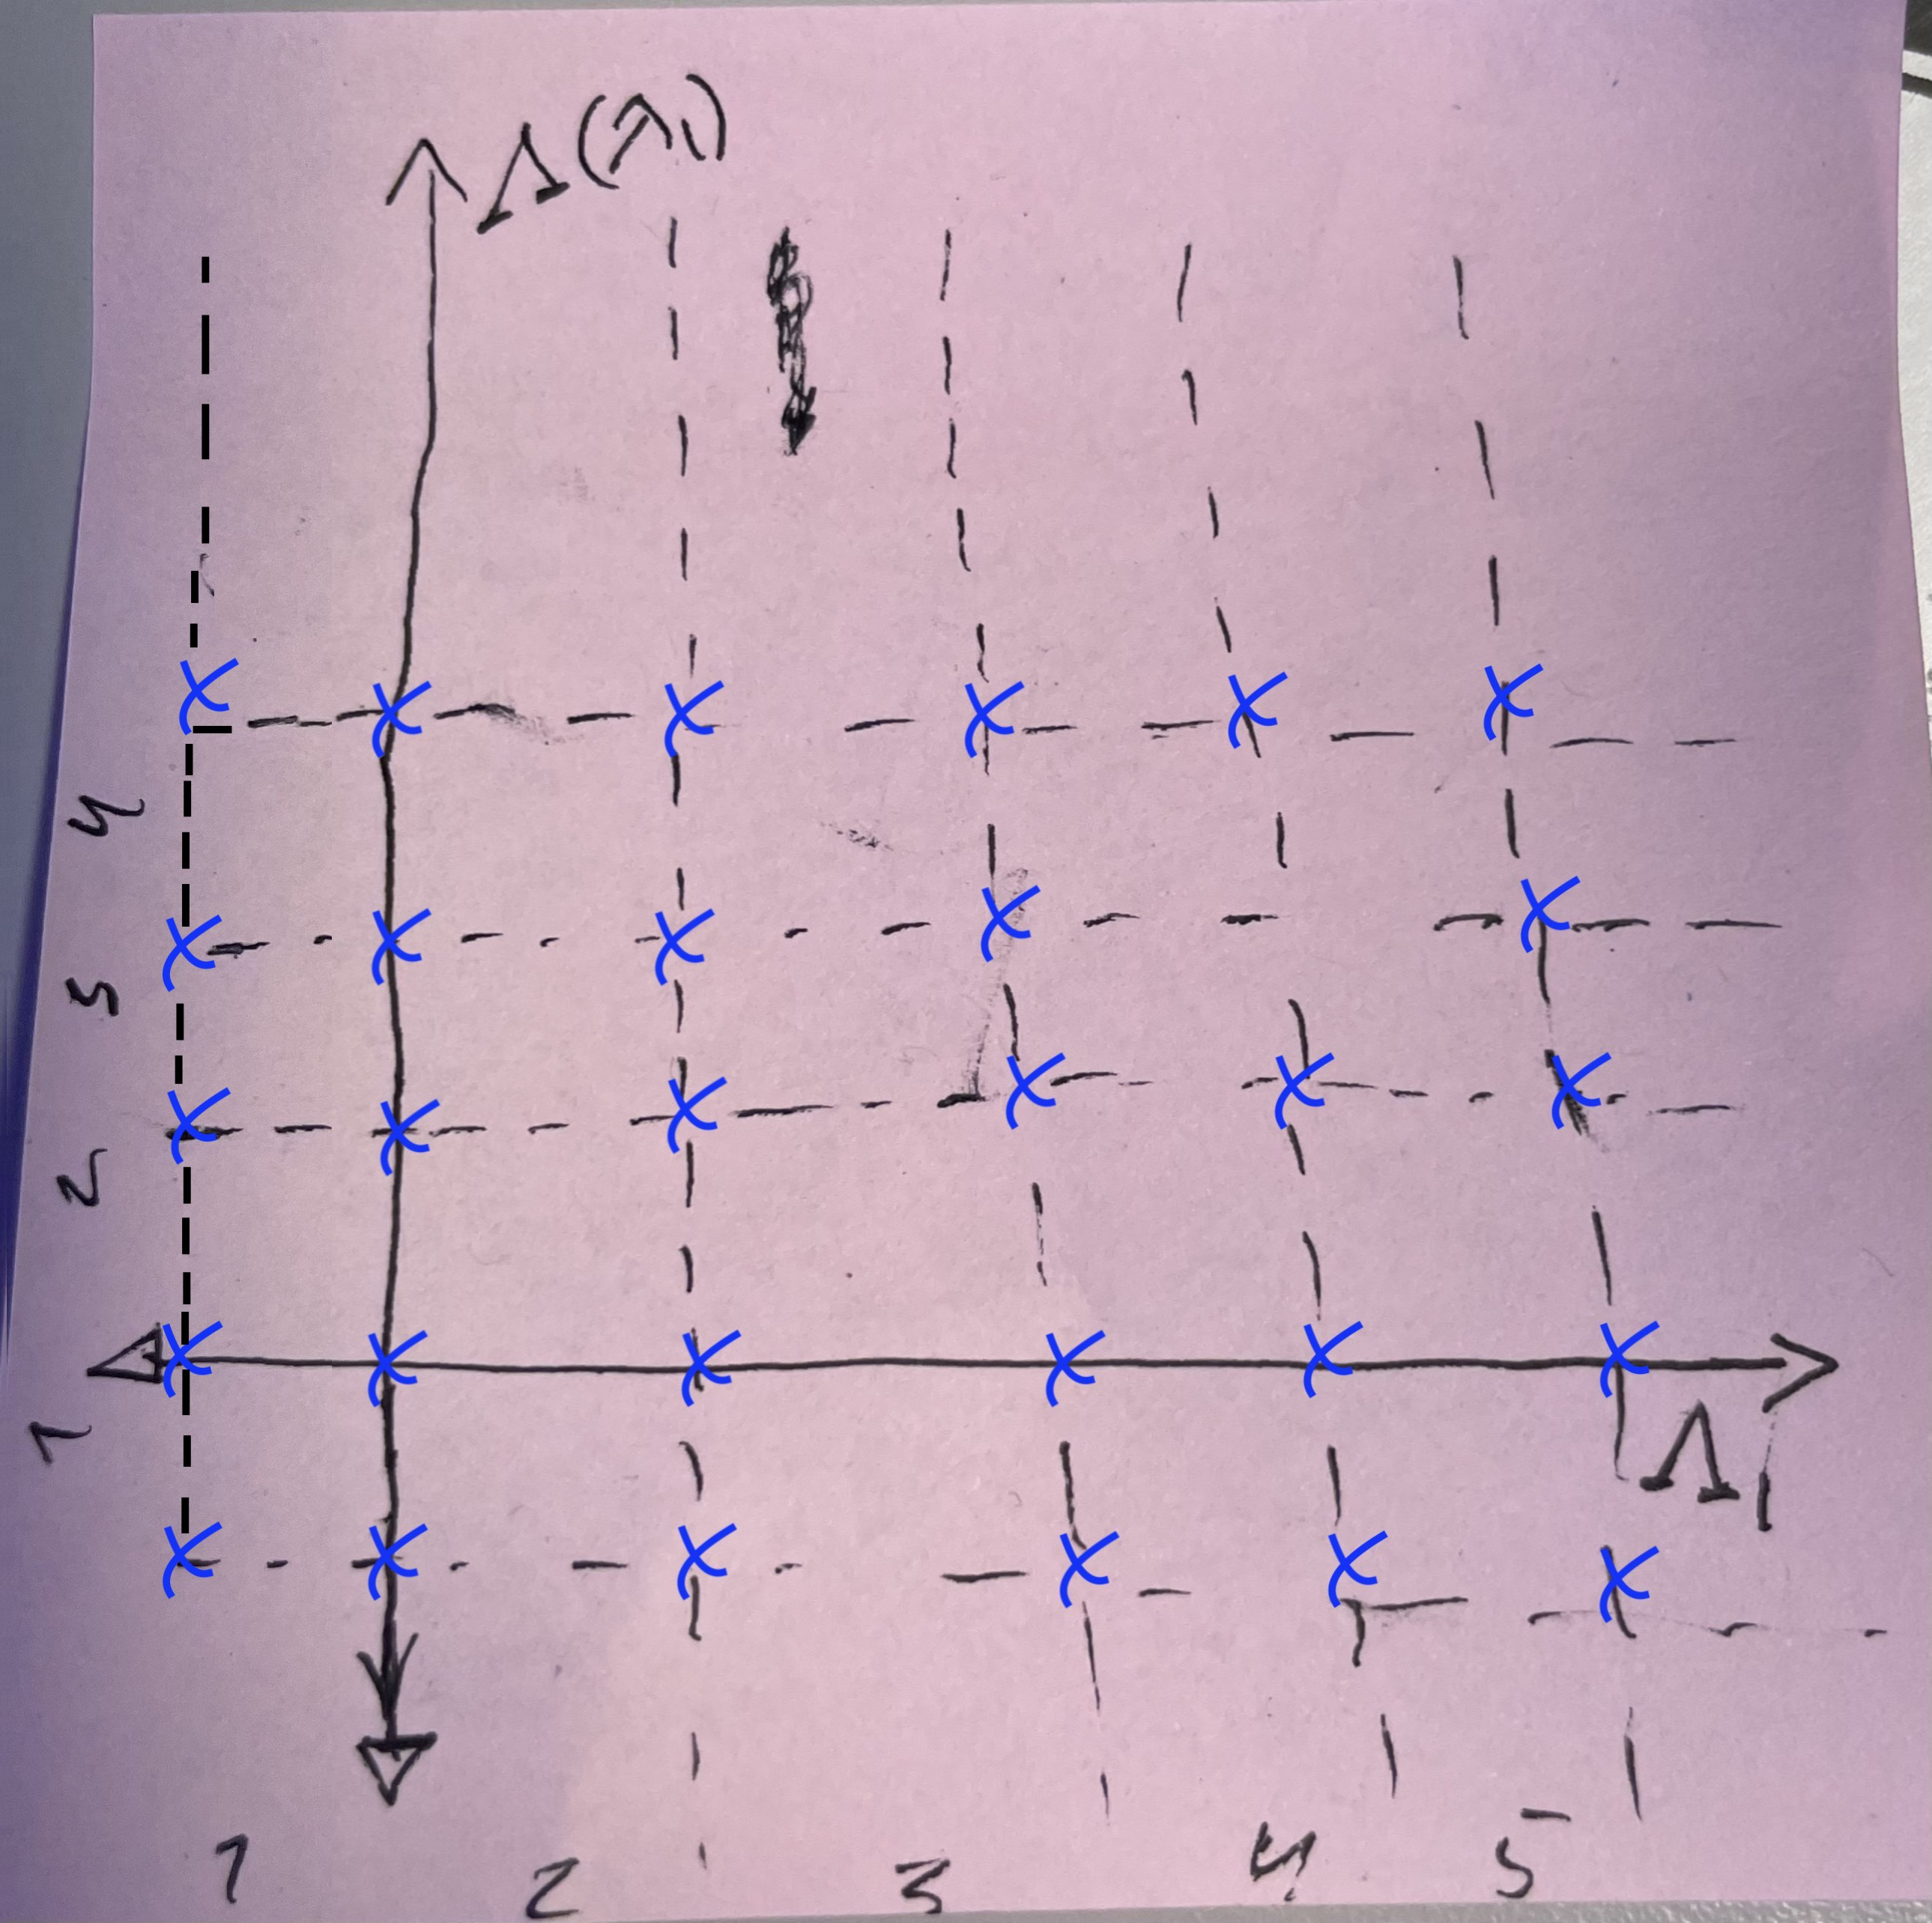
\includegraphics[width=0.9\linewidth]{spec_no_shift.jpg}
        %* Figure 1
        \begin{tikzpicture}[scale=1]
            % Define the tile
            \def\tile{
            \draw[fill=white] (0,0) rectangle (1,1);
            }
            \def\tiletwo{
            %\draw[black, fill=gray!65] (0,0) rectangle (1,1);
            %\draw[black, fill=cyan!65] (0,0) rectangle (1,1);
            \draw[pattern=north east lines, pattern color=MaxCyan4] (0,0) rectangle (1,1);
            }
            
            % Draw the tiling pattern
            % Shifted line, part 1, left and right half tiles 
            \foreach \x in {0}{
                %\draw[cyan, fill=cyan] (\x-0.2,2) rectangle (\x+0.5,3);  % leftmost value to the first square
                \draw[white, pattern=north east lines, pattern color=MaxCyan4] (\x-0.2,2) rectangle (\x+0.5,3); % leftmost value to the first square
            }
            \foreach \x in {6}{
                \draw[white, pattern=north east lines, pattern color=MaxCyan4] (\x+0.2,2) rectangle (\x-0.5,3);
                %\draw[gray!65, fill=cyan!65] (\x+0.2,2) rectangle (\x-0.5,3);  % rightmost value to the last square
            }
            % part 2, whole tiles in the middle
            % must be after the above code in order to get black lines at the correct spots
            \foreach \y in {2}{
                \foreach \x in {0,1,2,3,4}{
                    \pgfmathsetmacro{\shiftX}{\x+0.5} % Set horizontal shift
                    \pgfmathsetmacro{\shiftY}{\y}
                    \begin{scope}[shift={(\shiftX,\shiftY)}]
                        \tiletwo
                    \end{scope}
                }
            }
            % Everything else
            \foreach \y in {0,1,3,4}{
                \foreach \x in {0,1,2,3,4,5}{
                    \pgfmathsetmacro{\shiftX}{\x} % Set horizontal shift
                    \pgfmathsetmacro{\shiftY}{\y}
                    \begin{scope}[shift={(\shiftX,\shiftY)}]
                        \tile
                    \end{scope}
                }
            }
            % get the outline grid 
            



% small black lines at the left and right
\foreach \y in {0,1,2,3,4,5}{
    \draw (0-0.2,\y) -- (0,\y);  % Left
    \draw (6,\y) -- (6+0.2,\y);  % Right
    
}

% small black lines at the top and bottom
\foreach \x in {0,1,2,3,4,5,6}{
    \draw (\x,0-0.2) -- (\x,0);  % Top
    \draw (\x,5) -- (\x,5+0.2);  % Bottom
}
        \end{tikzpicture}
        %* —————————————————
        \caption{Single row shift}
        \label{fig:single_shift_horizontal_tiling}
    \end{subfigure}\quad
    \begin{subfigure}{.47\textwidth}
        \centering
        %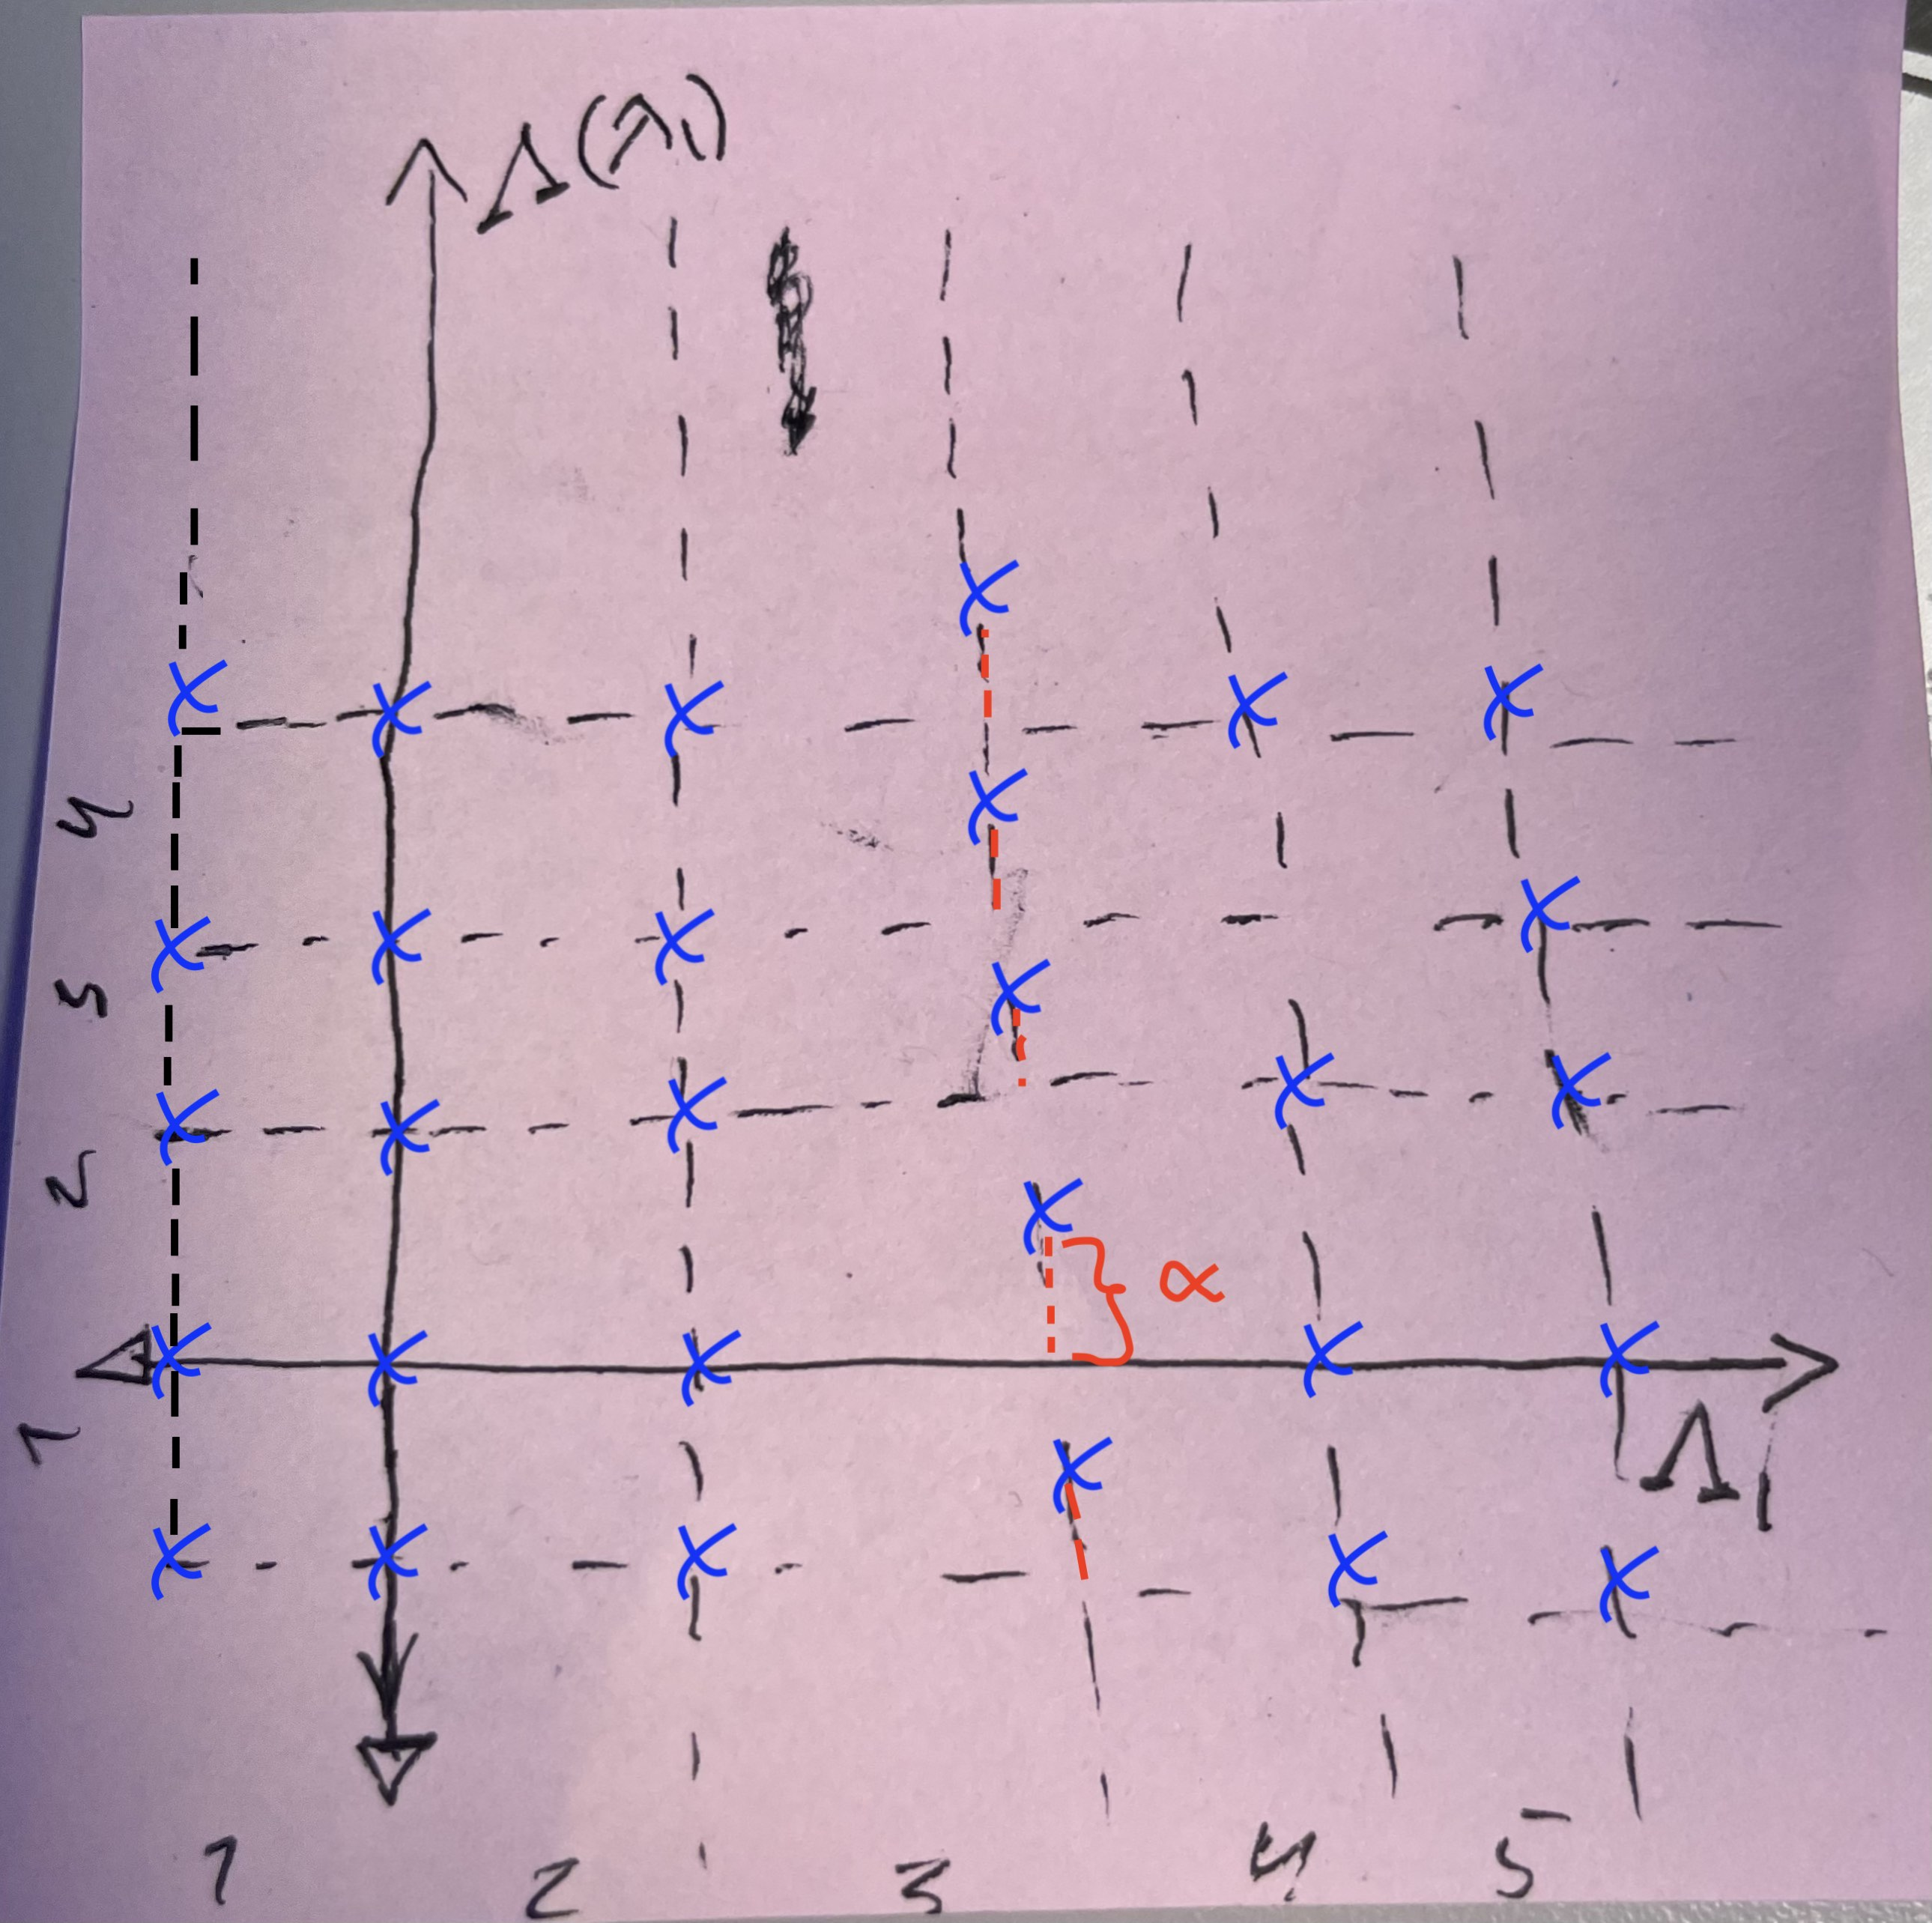
\includegraphics[width=0.9\linewidth]{spec_single_shift.jpg}
        %* Figure 2
        \begin{tikzpicture}[scale=1]
            % Define the tile
            \def\tile{
            \draw[fill=white] (0,0) rectangle (1,1);
            }
            \def\tiletwo{
            %\draw[fill=gray!65] (0,0) rectangle (1,1);
            %\draw[fill=YellowOrange] (0,0) rectangle (1,1);
            \draw[pattern=north east lines, pattern color=MaxOrange] (0,0) rectangle (1,1);
            }
            
            % Draw the tiling pattern
            % Shifted line, part 1, left and right half tiles 
            \foreach \y in {0}{
                %\draw[YellowOrange, fill=YellowOrange] (2,\y-0.2) rectangle (3,\y+0.5);
                \draw[white, pattern=north east lines, pattern color=MaxOrange] (2,\y-0.2) rectangle (3,\y+0.5);
                %\draw[orange!75, fill=orange!75] (2,\y-0.2) rectangle (3,\y+0.5);
            }
            \foreach \y in {5}{
                %\draw[YellowOrange, fill=YellowOrange] (2,\y+0.2) rectangle (3,\y-0.5);
                \draw[white, pattern=north east lines, pattern color=MaxOrange] (2,\y+0.2) rectangle (3,\y-0.5);
                %\draw[gray!65, fill=orange] (2,\y+0.2) rectangle (3,\y-0.5);
            }
            % part 2, whole tiles in the middle
            % must be after the above code in order to get black lines at the correct spots
            \foreach \x in {2}{
                \foreach \y in {0,1,2,3}{
                    \pgfmathsetmacro{\shiftX}{\x} % Set horizontal shift
                    \pgfmathsetmacro{\shiftY}{\y+0.5}
                    \begin{scope}[shift={(\shiftX,\shiftY)}]
                        \tiletwo
                    \end{scope}
                }
            }
            % Everything else
            \foreach \x in {0,1,3,4,5}{
                \foreach \y in {0,1,2,3,4}{
                    \pgfmathsetmacro{\shiftX}{\x} % Set horizontal shift
                    \pgfmathsetmacro{\shiftY}{\y}
                    \begin{scope}[shift={(\shiftX,\shiftY)}]
                        \tile
                    \end{scope}
                }
            }
            % get the outline grid 
            



% small black lines at the left and right
\foreach \y in {0,1,2,3,4,5}{
    \draw (0-0.2,\y) -- (0,\y);  % Left
    \draw (6,\y) -- (6+0.2,\y);  % Right
    
}

% small black lines at the top and bottom
\foreach \x in {0,1,2,3,4,5,6}{
    \draw (\x,0-0.2) -- (\x,0);  % Top
    \draw (\x,5) -- (\x,5+0.2);  % Bottom
}
        \end{tikzpicture}
        %* —————————————————
        \caption{Single column shift}
        \label{fig:single_shift_vertical_tiling}
    \end{subfigure}\\
    \begin{subfigure}{.47\textwidth}
        \centering
        %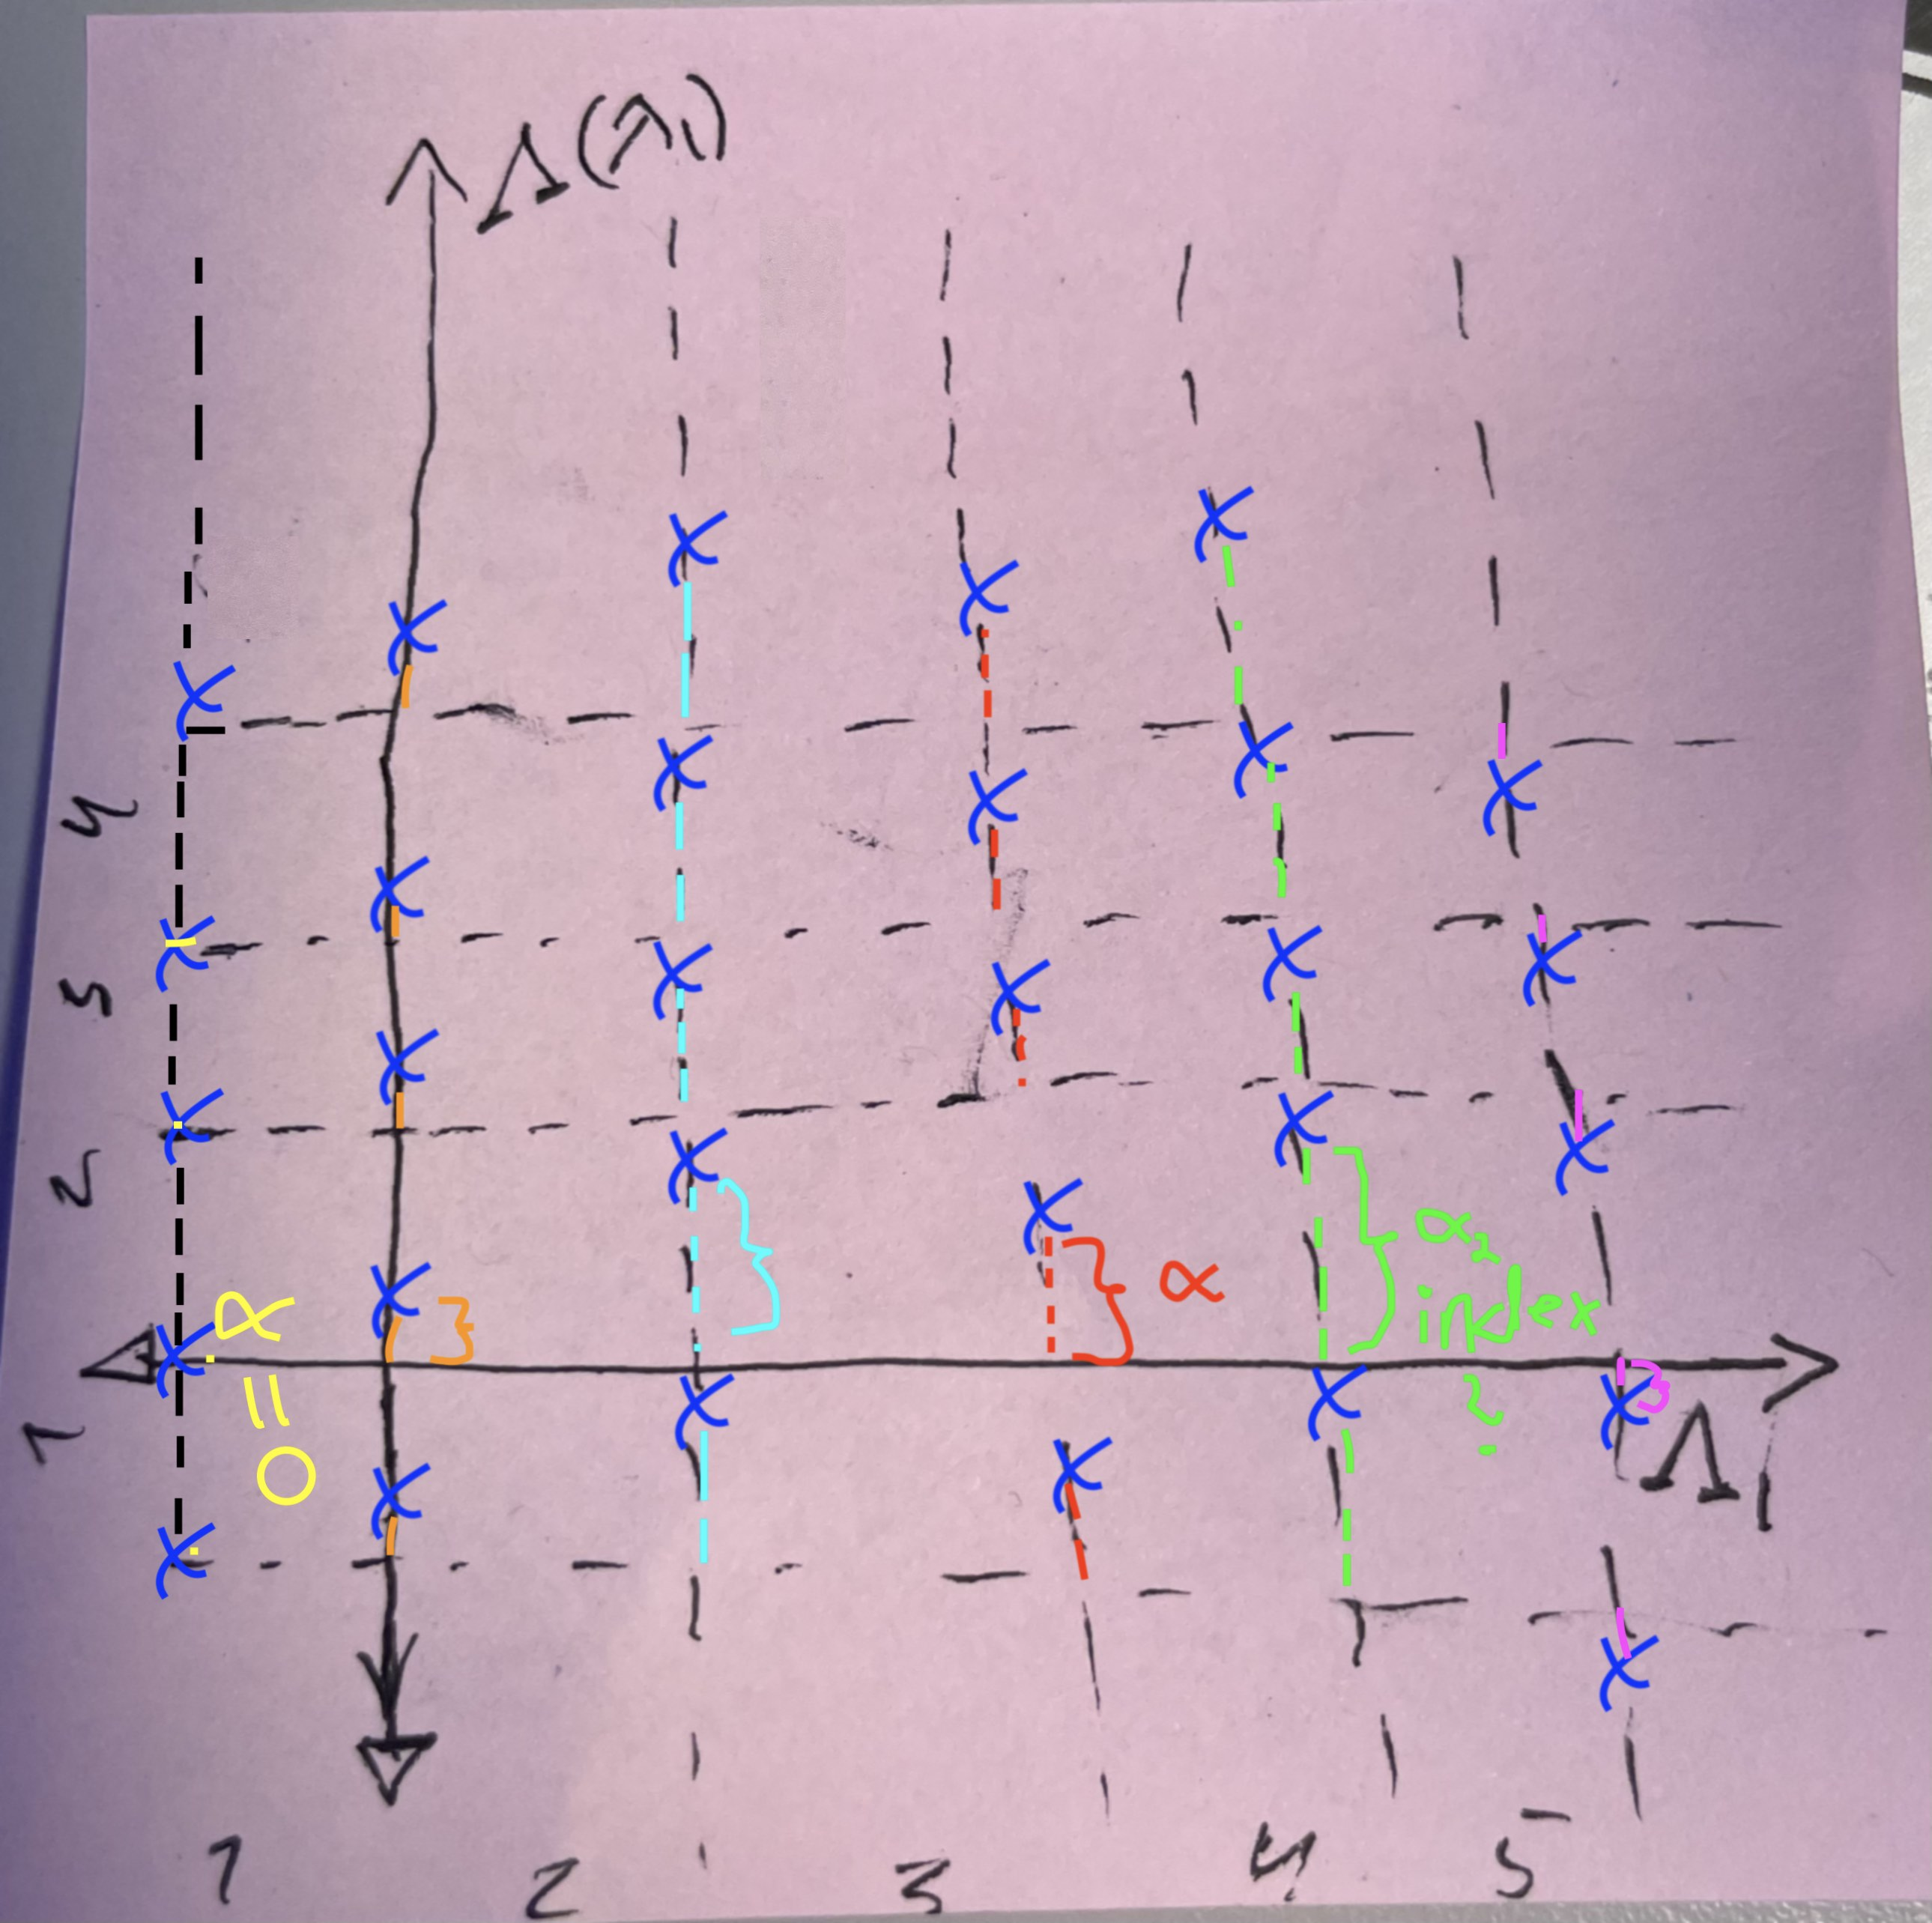
\includegraphics[width=0.9\linewidth]{multiple_shift_left_zero.jpg}
        %* Figure 3
        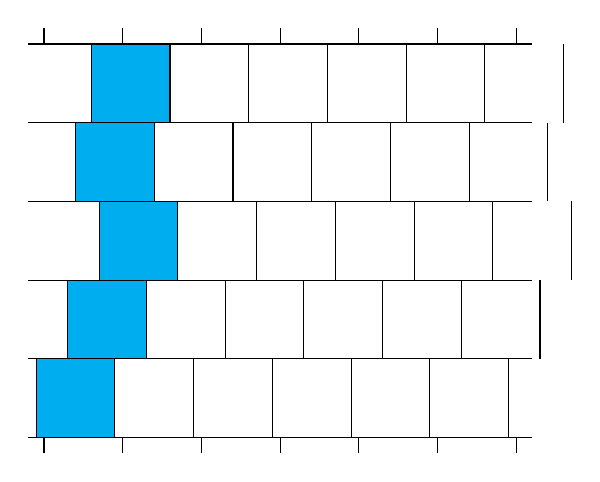
\begin{tikzpicture}[scale=1]
            % Define the tile
            \def\tile{
            % Draw the unit square
            \draw[fill=white] (0,0) rectangle (1,1);
            }
            \def\tiletwo{
            %\draw[fill=gray!65] (0,0) rectangle (1,1);
            \draw[fill=cyan] (0,0) rectangle (1,1);
            }

            % Shift list
            \def\BetaMinOne{-0.1}
            \def\BetaZero{0.3}
            \def\BetaOne{0.7}
            \def\BetaTwo{0.4}
            \def\BetaThree{0.6}
            
            % Draw the tiling pattern
            \foreach \x in {0,1,2,3,4}{
                \foreach \y in {0,1,2,3,4}{
                    \ifnum\y=0
                        \pgfmathsetmacro{\shiftX}{\x + \BetaMinOne}
                        \pgfmathsetmacro{\shiftY}{\y}
                        \pgfmathsetmacro{\shiftSingle}{\BetaMinOne}
                    \fi
                    \ifnum\y=1
                        \pgfmathsetmacro{\shiftX}{\x + \BetaZero}
                        \pgfmathsetmacro{\shiftY}{\y}
                        \pgfmathsetmacro{\shiftSingle}{\BetaZero}
                    \fi
                    \ifnum\y=2
                        \pgfmathsetmacro{\shiftX}{\x + \BetaOne} 
                        \pgfmathsetmacro{\shiftY}{\y} 
                        \pgfmathsetmacro{\shiftSingle}{\BetaOne}
                    \fi
                    \ifnum\y=3
                        \pgfmathsetmacro{\shiftX}{\x + \BetaTwo}
                        \pgfmathsetmacro{\shiftY}{\y}
                        \pgfmathsetmacro{\shiftSingle}{\BetaTwo}
                    \fi
                    \ifnum\y=4
                        \pgfmathsetmacro{\shiftX}{\x + \BetaThree}
                        \pgfmathsetmacro{\shiftY}{\y}
                        \pgfmathsetmacro{\shiftSingle}{\BetaThree}
                    \fi
                    % Drawing the left half-cubes
                    \ifnum\x=0
                        \draw[white, fill=white](\x-0.2,\y) rectangle (\x+\shiftSingle,\y+1);
                    \fi
                    % Drawing the right half-cubes
                    \ifnum\x=4
                        \ifthenelse{\lengthtest{\shiftSingle pt > 0.2 pt}}{
                            \draw[white] (\x+2+\shiftSingle,\y+1) -- (\x+2+\shiftSingle,\y);  % Right line
                        }{
                            \draw[black] (\x+2+\shiftSingle,\y+1) -- (\x+2+\shiftSingle,\y);  % Right line
                        }
                        %\draw[black] (\x+1,\y) -- (\x,\y+2);  % Left line
                        %\draw[black] (\x+2+\shiftSingle,\y) -- (\x+2+\shiftSingle,\y+1);  % Top
                        %\draw[black] (\x+1+\shiftSingle,\y+1) -- (\x+1+\shiftSingle,\y);  % Bottom line
                    \fi
                    % Drawing the rest of the middle cubes
                    \begin{scope}[shift={(\shiftX,\shiftY)}]
                        \tile % Draw the tile
                    \end{scope}
                    % Drawing a new line of shifted colored cubes on top at the first row
                    \ifnum\x=0
                    \begin{scope}[shift={(\shiftX,\shiftY)}]
                        \tiletwo
                    \end{scope}
                    \fi
                }   
            }
            % get the outline grid 
            % small black lines at the left and right
            \foreach \y in {0,1,2,3,4,5}{
                %\draw (0-0.2,\y) -- (0,\y);  % Left
                %\draw (6,\y) -- (6+0.2,\y);  % Right
                \draw (0-0.2,\y) -- (6+0.2,\y);  % Right
            }
            
            % small black lines at the top and bottom
            \foreach \x in {0,1,2,3,4,5,6}{
                \draw (\x,0-0.2) -- (\x,0);  % Top
                \draw (\x,5) -- (\x,5+0.2);  % Bottom
            }
        \end{tikzpicture}
        %* —————————————————
        \caption{Multiple row shifts}
        \label{fig:multiple_shift_horizontal_tiling}
    \end{subfigure}\quad
    \begin{subfigure}{.47\textwidth}
        \centering
        %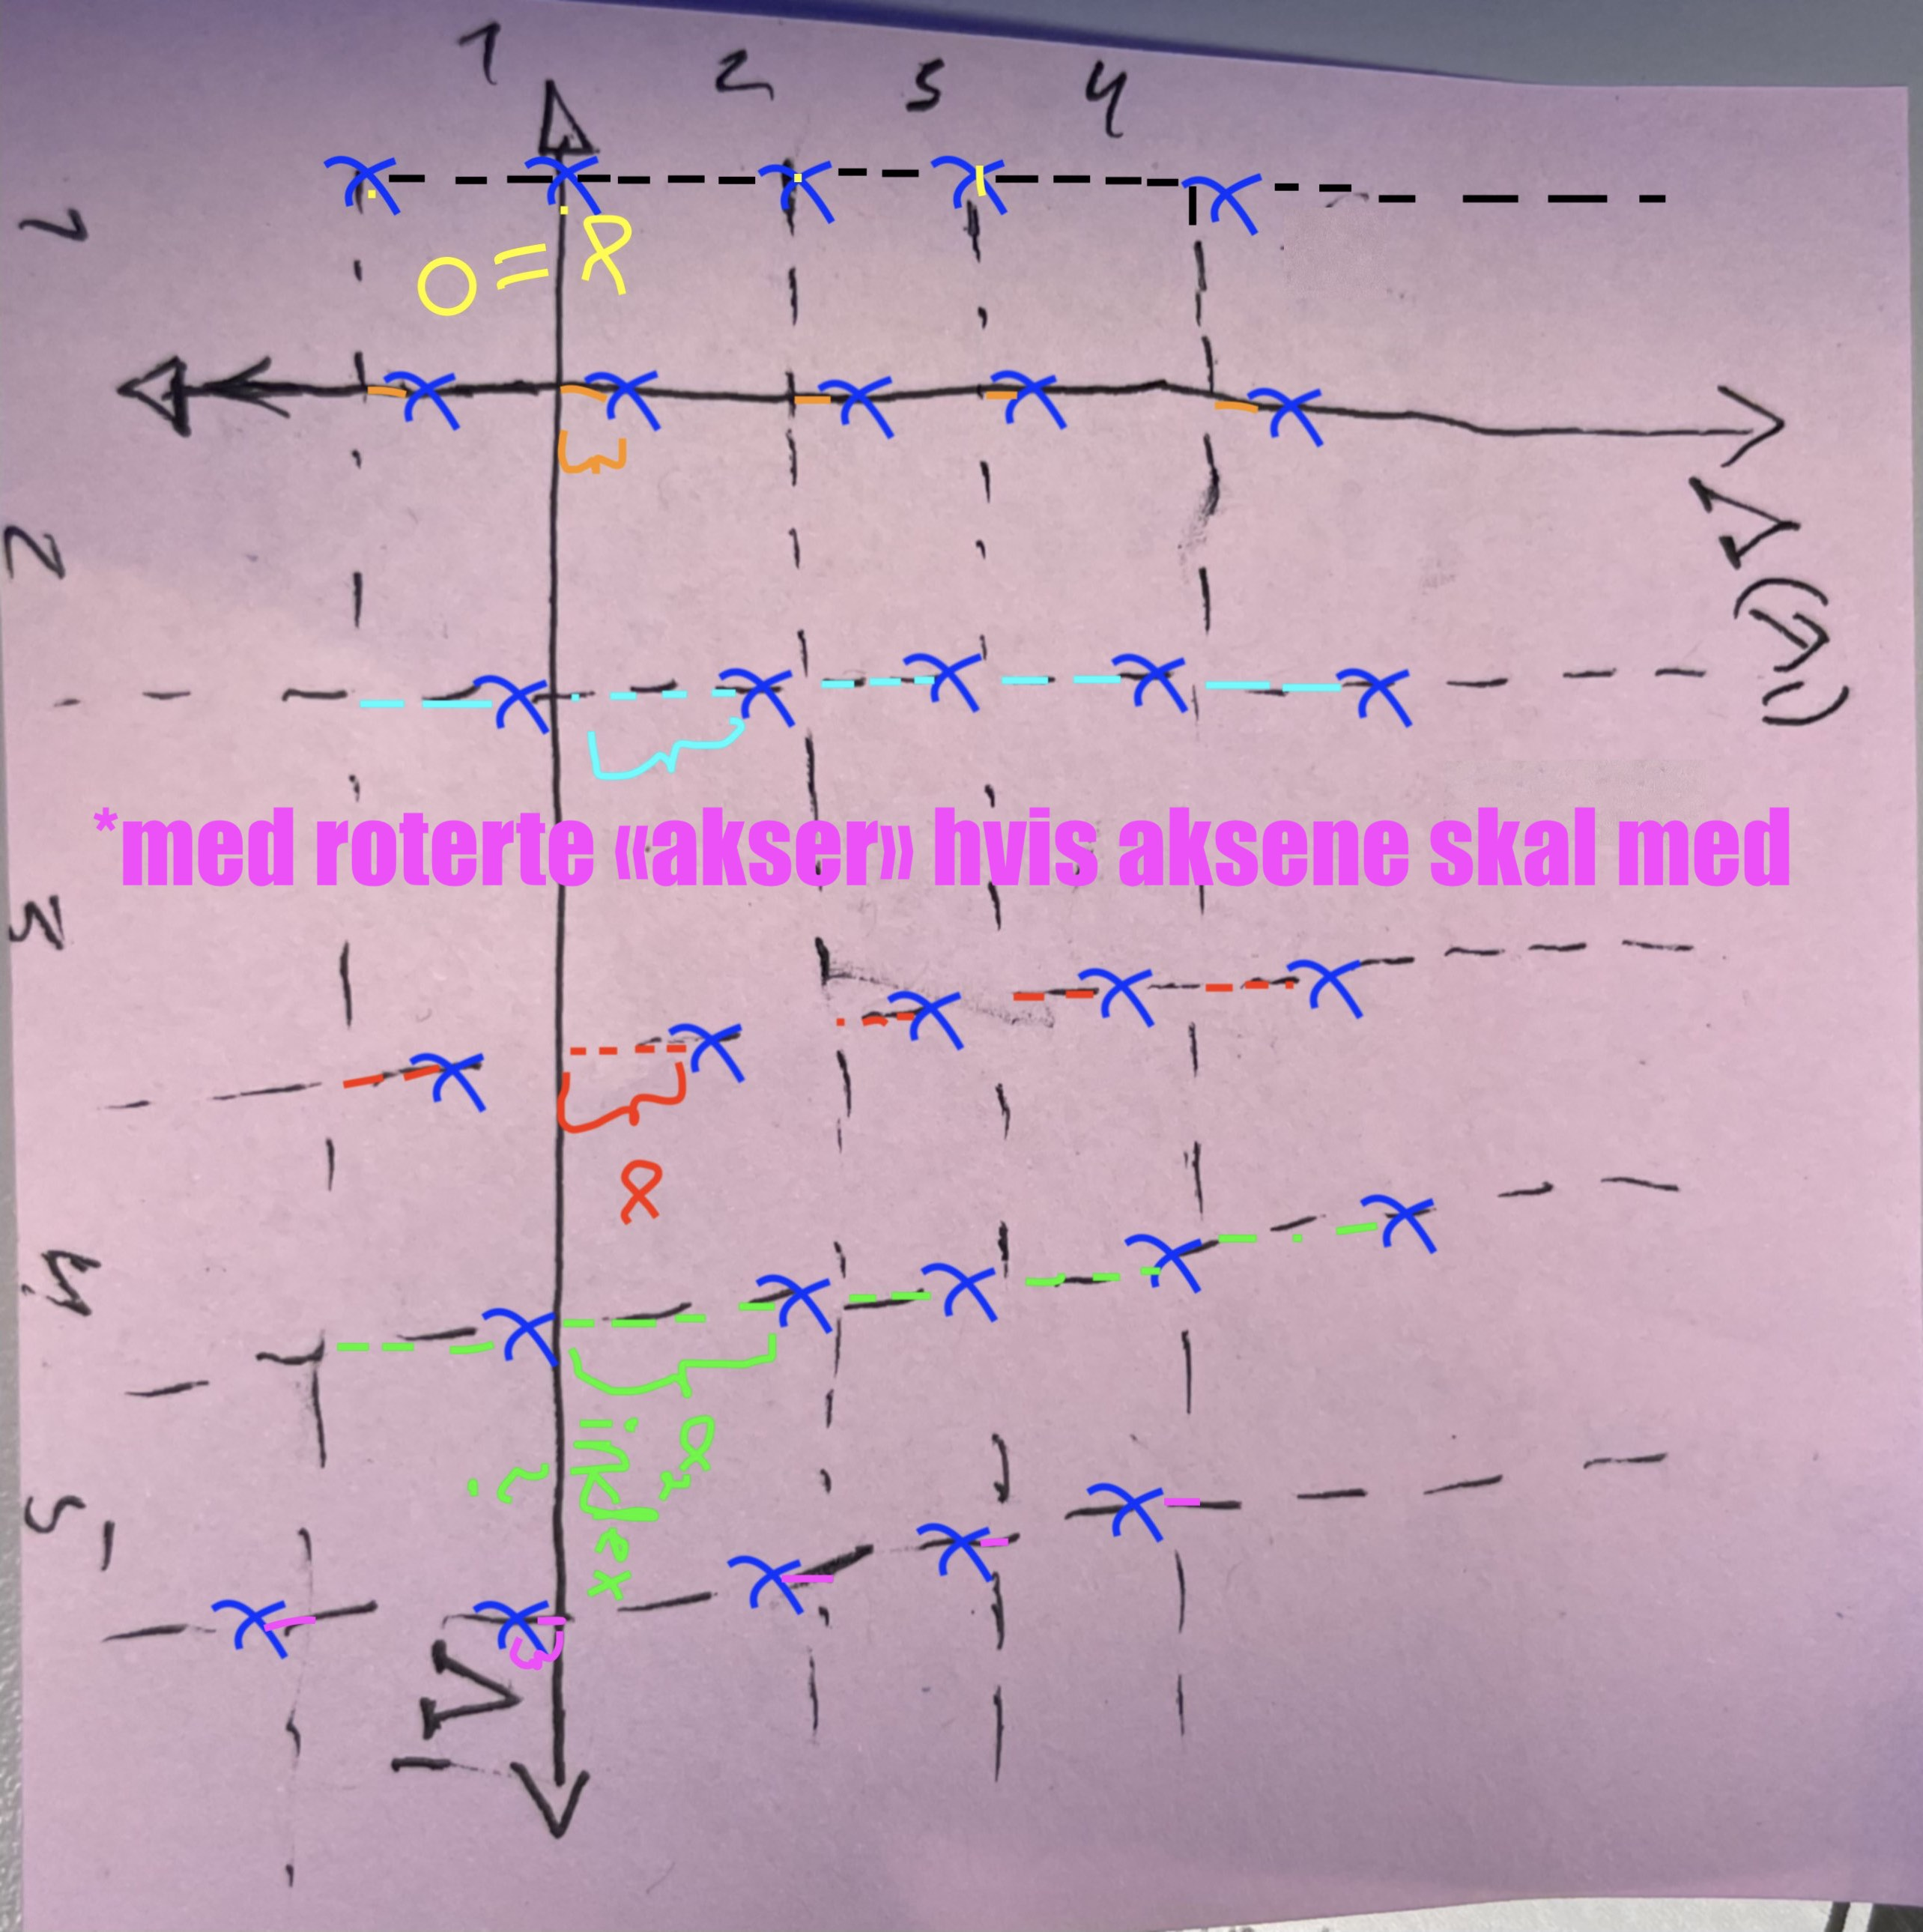
\includegraphics[width=0.9\linewidth]{multiple_shift_left_zero_horizontal.jpg}
        %* Figure 4
        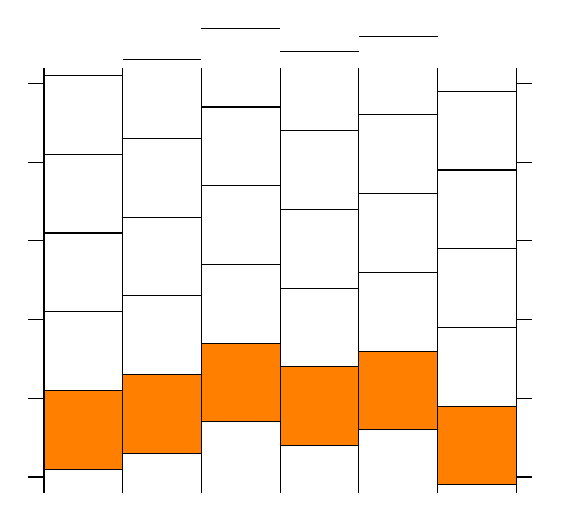
\begin{tikzpicture}[scale=1]
            % Define the tile
            \def\tile{
            % Draw the unit square
            \draw[fill=white] (0,0) rectangle (1,1);
            }
            \def\tiletwo{
            %\draw[fill=gray!65] (0,0) rectangle (1,1);
            \draw[fill=orange] (0,0) rectangle (1,1);
            %\draw[->] (0.5,0) -- (0.5,0.9);  % If arrows from the middle
            }

            % Shift list
            \def\BetaMinOne{0.1}
            \def\BetaZero{0.3}
            \def\BetaOne{0.7}
            \def\BetaTwo{0.4}
            \def\BetaThree{0.6}
            \def\BetaFour{-0.1}

            % Draw the tiling pattern
            \foreach \x in {0,1,2,3,4,5}{
                \foreach \y in {0,1,2,3}{
                    \ifnum\x=0
                        \pgfmathsetmacro{\shiftX}{\x}
                        \pgfmathsetmacro{\shiftY}{\y + \BetaMinOne}
                        \pgfmathsetmacro{\shiftSingle}{\BetaMinOne}
                    \fi
                    \ifnum\x=1
                        \pgfmathsetmacro{\shiftX}{\x}
                        \pgfmathsetmacro{\shiftY}{\y + \BetaZero}
                        \pgfmathsetmacro{\shiftSingle}{\BetaZero}
                    \fi
                    \ifnum\x=2
                        \pgfmathsetmacro{\shiftX}{\x} 
                        \pgfmathsetmacro{\shiftY}{\y + \BetaOne} 
                        \pgfmathsetmacro{\shiftSingle}{\BetaOne}
                    \fi
                    \ifnum\x=3
                        \pgfmathsetmacro{\shiftX}{\x}
                        \pgfmathsetmacro{\shiftY}{\y + \BetaTwo}
                        \pgfmathsetmacro{\shiftSingle}{\BetaTwo}
                    \fi
                    \ifnum\x=4
                        \pgfmathsetmacro{\shiftX}{\x}
                        \pgfmathsetmacro{\shiftY}{\y + \BetaThree}
                        \pgfmathsetmacro{\shiftSingle}{\BetaThree}
                    \fi
                    \ifnum\x=5
                        \pgfmathsetmacro{\shiftX}{\x}
                        \pgfmathsetmacro{\shiftY}{\y + \BetaFour}
                        \pgfmathsetmacro{\shiftSingle}{\BetaFour}
                    \fi
                    % Drawing the bottom half-cubes
                    \ifnum\y=0
                        \draw[white, fill=white](\x,\y-0.2) rectangle (\x+1,\y+\shiftSingle);
                    \fi
                    % Drawing the top half-cubes
                    \ifnum\y=3
                        \ifthenelse{\lengthtest{\shiftSingle pt > 0.2 pt}}{
                            \draw[white] (\x,\y+2+\shiftSingle) -- (\x+1,\y+2+\shiftSingle);  % Top
                        }{
                        \draw[black] (\x,\y+2+\shiftSingle) -- (\x+1,\y+2+\shiftSingle);  % Top
                        }
                        \draw[black] (\x,\y+1) -- (\x,\y+2);  % Left line
                        \draw[black] (\x+1,\y+2) -- (\x+1,\y+1);  % Right line
                        \draw[black] (\x+1,\y+1+\shiftSingle) -- (\x,\y+1+\shiftSingle);  % Bottom line
                        %\draw[red, fill=red](\x,\y+1) rectangle (\x+1,\y+2);
                    \fi
                    % Drawing the rest of the middle cubes
                    \begin{scope}[shift={(\shiftX,\shiftY)}]
                        \tile
                    \end{scope}
                    % Drawing a new line of shifted colored cubes on top at the first row
                    \ifnum\y=0
                        \begin{scope}[shift={(\shiftX,\shiftY)}]
                            \tiletwo
                        \end{scope}
                    \fi
                }  
            }
            % get the outline grid 
            % small black lines at the left and right
            \foreach \y in {0,1,2,3,4,5}{
                \draw (0-0.2,\y) -- (0,\y);  % Left
                \draw (6,\y) -- (6+0.2,\y);  % Right
            }
            % small black lines at the top and bottom
            \foreach \x in {0,1,2,3,4,5,6}{
                %\draw (\x,0-0.2) -- (\x,0);  % Top
                %\draw (\x,5) -- (\x,5+0.2);  % Bottom
                \draw (\x,0-0.2) -- (\x,5+0.2);  % Shift only in the vertical direction, therefore only one line
            }
        \end{tikzpicture}
        %* —————————————————
        \caption{Multiple column shifts}
        \label{fig:multiple_shift_vertical_tiling}
    \end{subfigure}
    \caption{Illustration of four tiling pairs for $\brac{I^2,\Lambda}$ covering $\R^2$. The cyan and orange colors represent shifts in the horizontal and vertical direction, respectively. The dashed line pattern in \cref{fig:single_shift_horizontal_tiling,fig:single_shift_vertical_tiling} highlights the single row or column which is shifted, and the filled cubes in \cref{fig:multiple_shift_horizontal_tiling,fig:multiple_shift_vertical_tiling} highlights the different shifts used for each row or column. Note that if this were a lattice tiling, all the cyan-filled or orange-filled squares would be on the same vertical or horizontal line, respectively.}
    \label{fig:tiling_figures}
\end{figure}

%\extractcolorspecs{Cyan}{\myColorModel}{\myColor} orange is \myColor\ in model %\myColorModel

\end{document}